\chapter{Making the most of your data - Data Augmentation and Transfer Learning}

\section{Data Augmentation}

\subsection*{Horizontal Flip} 
\begin{figure}[!htb]
  \centering
  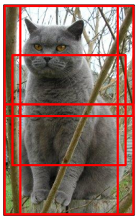
\includegraphics[width=0.125\textwidth]{Images/data_aug_trans/1.png}
  \caption{Horizontal flip. Flip image 180 degrees in the horizontal direction.}
\end{figure}


\subsection*{Random Crops/Scales}
\begin{figure}[!htb]
  \centering
  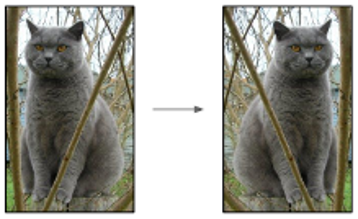
\includegraphics[width=0.3\textwidth]{Images/data_aug_trans/2.png}
  \caption{Random Crops/Scales}
\end{figure}

\textbf{Training}: sample random crops / scales

Specific example. How ResNet trains:
\begin{enumerate}
\item Pick random L in range [256, 480]
\item Resize training image, short side = L
\item Sample random 224 x 224 patch
\end{enumerate}

\textbf{Testing}: average a fixed set of crops 

Specific example. How ResNet tests:
\begin{enumerate}
\item Resize image at 5 scales: {224, 256, 384, 480, 640}
\item For each size, use 10 224 x 224 crops: 4 corners + center, + flips
\end{enumerate}

\subsection*{Color Jitter}
\begin{figure}[!htb]
  \centering
  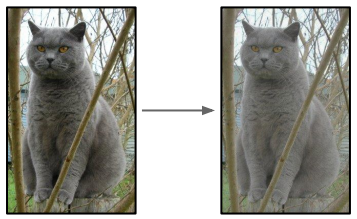
\includegraphics[width=0.3\textwidth]{Images/data_aug_trans/3.png}
  \caption{Color Jitter}
\end{figure}
\begin{itemize}
\item Simple: Randomly jitter contrast

\item Complex:
\begin{enumerate}
\item Apply PCA to all [R, G, B] pixels in training set
\item Sample a “color offset” along principal component directions
\item Add offset to all pixels of a training image
\end{enumerate}
\end{itemize}

\subsection*{Get Creative}
At the end you have to think for your specific case, what transformations you want to be robust to and add them to the training set: translation, 
rotation, stretching, shearing, lens distortions, ...


\section{Transfer Learning}
In practice, very few people train an entire Deep Network from scratch (with random initialization), because it is relatively rare to have a dataset of sufficient size. Instead, it is common to pretrain a ConvNet on a very large dataset (e.g. ImageNet, which contains 1.2 million images with 1000 categories), and then use the ConvNet either as an initialization or a fixed feature extractor for the task of interest. Pretrained DeepNets are usually trained with large computer clusters and downloaded by others. The three major Transfer Learning scenarios look as follows:

\paragraph*{ConvNet as fixed feature extractor} Take a ConvNet pretrained on ImageNet, remove the last fully-connected layer (this layer’s outputs are the 1000 class scores for a different task like ImageNet), then treat the rest of the ConvNet as a fixed feature extractor for the new dataset. In an AlexNet, this would compute a 4096-D vector for every image that contains the activations of the hidden layer immediately before the classifier. We call these features CNN codes. 
\paragraph*{Fine-tuning the ConvNet} The second strategy is not only to replace and retrain the classifier on top of the ConvNet on the new dataset, but to also fine-tune the weights of the pretrained network by continuing the backpropagation. It is possible to fine-tune all the layers of the ConvNet, or it’s possible to keep some of the earlier layers fixed (due to overfitting concerns) and only fine-tune some higher-level portion of the network. This is motivated by the observation that the earlier features of a ConvNet contain more generic features (e.g. edge detectors or color blob detectors) that should be useful to many tasks, but later layers of the ConvNet becomes progressively more specific to the details of the classes contained in the original dataset. In case of ImageNet for example, which contains many dog breeds, a significant portion of the representational power of the ConvNet may be devoted to features that are specific to differentiating between dog breeds.

\paragraph*{Check points of pretrained models} Since modern ConvNets take 2-3 weeks to train across multiple GPUs on ImageNet, it is common to see people release their final ConvNet checkpoints for the benefit of others who can use the networks for fine-tuning. For example, the Caffe library has a Model Zoo where people share their network weights.

\subsection*{When and how to fine-tune?}
\begin{figure}[!htb]
  \centering
  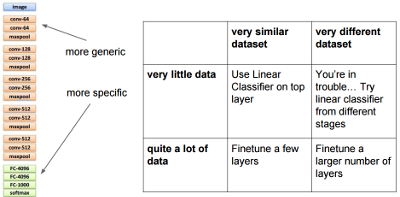
\includegraphics[width=0.6\textwidth]{Images/data_aug_trans/4.png}
  \caption{Random Crops/Scales}
\end{figure}
IMPORTANT: When doing transfer learning if you make changes in the green and orange part do the following:
\begin{itemize}
\item Train green, freeze everything else
\item When green is starting to converge unfreeze the orange part that you want to modify
\end{itemize}

This is necessary because green starts with random values and it may produce very big gradients that may destroy your previous layers

\subsection*{Practical advice}
There are a few additional things to keep in mind when performing Transfer Learning:

\paragraph*{Constraints from pretrained models} Note that if you wish to use a pretrained network, you may be slightly constrained in terms of the architecture you can use for your new dataset. For example, you can’t arbitrarily take out Conv layers from the pretrained network. However, some changes are straight-forward: Due to parameter sharing, you can easily run a pretrained network on images of different spatial size. This is clearly evident in the case of Conv/Pool layers because their forward function is independent of the input volume spatial size (as long as the strides “fit”). In case of FC layers, this still holds true because FC layers can be converted to a Convolutional Layer: For example, in an AlexNet, the final pooling volume before the first FC layer is of size [6x6x512]. Therefore, the FC layer looking at this volume is equivalent to having a Convolutional Layer that has receptive field size 6x6, and is applied with padding of 0.

\paragraph*{Learning rates} It’s common to use a smaller learning rate for ConvNet weights that are being fine-tuned, in comparison to the (randomly-initialized) weights for the new linear classifier that computes the class scores of your new dataset. This is because we expect that the ConvNet weights are relatively good, so we don’t wish to distort them too quickly and too much (especially while the new Linear Classifier above them is being trained from random initialization).